\documentclass[titlepage]{article}[12pt] 
\usepackage{braket}
\usepackage[margin=1in]{geometry}
\usepackage{amsmath}
\usepackage{pgfplots}
\usepackage{float}
\usepackage{soul}
\pgfplotsset{compat=newest}
\usepackage{tikz} 
\usepackage{circuitikz}
\usepackage{titlesec}

\usepackage{mathtools} % for 'bsmallmatrix' environment
\newenvironment{brsm}{% % short for 'bracketed small matrix'
  \bigl[ \begin{smallmatrix} }{%
  \end{smallmatrix} \bigr]}


\usepackage[style=verbose,bibstyle=numeric,sorting=none,backend=bibtex]{biblatex}
\addbibresource{Final.bib}



\setcounter{secnumdepth}{4}
\titleformat{\paragraph}
{\normalfont\normalsize\bfseries}{\theparagraph}{1em}{}
\titlespacing*{\paragraph}
{0pt}{3.25ex plus 1ex minus .2ex}{1.5ex plus .2ex}
\titlespacing\section{0pt}{12pt plus 4pt minus 2pt}{5pt plus 2pt minus 2pt}
\titlespacing\subsection{0pt}{12pt plus 4pt minus 2pt}{5pt plus 2pt minus 2pt}
\titlespacing\subsubsection{0pt}{12pt plus 4pt minus 2pt}{5pt plus 2pt minus 2pt}
\begin{document}
\title{To What Extent Could Quantum Computers Improve On Classical Computers?}
\author{Sam Robbins\\The King Edward VI School, Morpeth}
\renewcommand{\today}{}
\maketitle 
\tableofcontents
\newpage
\section{Introduction}
Quantum computing is a key concept in computing, as it is a method which allows for far faster computing, beyond the current limits of classical computing. My question is: to what extent could quantum computers improve on classical computers. I chose this topic because of its relevance to the future of computing and the impact it can have on the world. I am particularly interested in it due to my future plans to study Computer Science at university and my interest in Physics. 

I am going to explore this subject by finding out the key ways in which quantum computers improve on classical computers, and compare the way a quantum computer carries out a process compared to a classical computer. After this I will compare the two methods, finding which is the best. I will also compare the hardware of both quantum and classical computers, comparing them and finding which scenarios each perform best in 
\\
Quantum computers are computers that work on a superposition of states, rather than the 1 and 0 as classical computers do. This allows for them to process data much faster due to more efficient algorithms able to utilise the larger number of states, alongside quantum properties such as entanglement. I will be comparing these to classical computers, which have been developed over a much longer time, allowing for the most efficient algorithms on that hardware to be created, however these can't be developed much further due to the physical limitations of classical computers.

\section{The Physics of Computers}
\subsection{The physics of classical computers}
\subsubsection{Transistors}
Classical computers work using transistors, these are in effect electronic switches which will either permit or deny current through them based on the current in the third leg.
   \begin{figure}[H]
\begin{center}
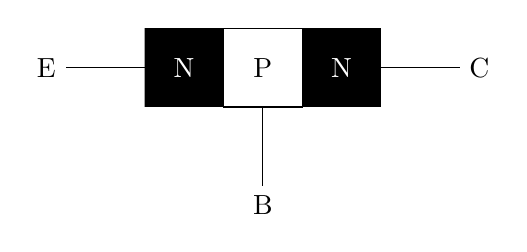
\begin{tikzpicture}
\fill[black!100] (0,0) -- (1,0) -- (1,1) -- (0,1) -- (0,0);
\draw (1,0) -- (2,0) -- (2,1) -- (1,1) -- (1,0);
\fill[black!100] (2,0) -- (3,0) -- (3,1) -- (2,1) -- (2,0);
\draw (0,0.5) -- (-1,0.5);
\draw (3,0.5) -- (4,0.5);
\draw (1.5,0) -- (1.5,-1);
\node[draw,text=white] at (0.5,0.5) {N};
\node[fill=white] at (1.5,0.5) {P};
\node[draw,text=white] at (2.5,0.5) {N};
\node[] at (-1.25,0.5) {E};
\node[] at (4.25,0.5) {C};
\node[] at (1.5,-1.25) {B};
\end{tikzpicture}
\end{center}
\centering 
\caption{PNP Transistor}
\end{figure} 
In this diagram the electrons are collected at the collector (C) and then taken into the N doped silicon. When electrons are provided to the base (B) they will flow into the P doped silicon. This will then cause electrons to flow from the collector to the emitter (E), producing a current.
\subsubsection{Transistors and Logic Gates}
Transistors can be arranged in many ways to produce logic gates. These are then used in various combinations to perform the mathematical operations that are used in classical algorithms.
\begin{figure}[H]
  \begin{center}
    \begin{circuitikz}
   \draw (0,0) node[npn](npn1) {}
  (npn1.base) node[anchor=east] {}
  (npn1.collector) node[anchor=south] {+}
  (npn1.emitter) node[anchor=north] {};
  \draw (0,-2) node[npn](npn2) {}
  (npn2.base) node[anchor=east] {}
  (npn2.collector) node[anchor=south] {}
  (npn2.emitter) node[anchor=north] {};
  \draw (npn1.emitter) to[short] (npn2.collector);
  \draw (npn1.base) to[short] (npn2.base);
  \draw (0,-1) to[short]node[anchor=west] {Y} (1,-1);
  \draw (-0.8,-1) to[short] node[anchor=east]{X} (-2,-1);
    \end{circuitikz}
    \caption{NOT Gate}
  \end{center}
\end{figure}
Above is shown the NOT gate, constructed from transistors, the input, X, will be inverted to Y.

\begin{figure}[H]
  \begin{center}
    \begin{circuitikz}
   \draw (0,0) node[npn](npn1) {}
  (npn1.base) node[anchor=east] {X}
  (npn1.collector) node[anchor=south] {+}
  (npn1.emitter) node[anchor=north] {};
  \draw (0,-2) node[npn](npn2) {}
  (npn2.base) node[anchor=east] {Y}
  (npn2.collector) node[anchor=south] {}
  (npn2.emitter) node[anchor=north] {Z};
  \draw (npn1.emitter) to[short] (npn2.collector);
    \end{circuitikz}
    \caption{AND Gate}
  \end{center}
\end{figure}
Above is the AND gate, this requires both X and Y to be on, in order for Z to be on. This is because when X is on it will provide current for Transistor 2, which will only transmit if Y is on.
\begin{figure}[H]
  \begin{center}
    \begin{circuitikz}
   \draw (0,0) node[npn](npn1) {}
  (npn1.base) node[anchor=east] {X}
  (npn1.collector) node[anchor=south] {}
  (npn1.emitter) node[anchor=north] {};
  \draw (0,-2) node[npn](npn2) {}
  (npn2.base) node[anchor=east] {Y}
  (npn2.collector) node[anchor=south] {}
  (npn2.emitter) node[anchor=north] {};
  \draw (0,0.7) to[short,*-*] node[anchor=east]{} (1,0.7);
  \draw (0,-1.3) to[short,*-*] node[anchor=east]{} (1,-1.3);
  \draw (1,1.5) node[label={[font=\footnotesize]above:+}] {} to[short,*-*] node[anchor=east]{} (1,-1.3);
  \draw (2,-0.7) to[short] node[anchor=east]{} (2,-3);
  \draw (2,-3) to[R] node[ground]{GND}  (2,-5);
  \draw (0,-0.7) to[short,*-*] node[anchor=east]{} (2,-0.7);
  \draw (0,-2.7) to[short,*-*] node[anchor=east]{} (2,-2.7);
  \draw (2,-2.7) to[short,*-*] node[anchor=east]{}  (3,-2.7)node[label={[font=\footnotesize]east:Z}] {};
    \end{circuitikz}
    \caption{OR Gate}
  \end{center}
\end{figure}
Above is the OR gate, the collectors of the transistors are connected to the + node, so that whenever the base (X or Y) receives an input, it will give an output to the collector. The collector of both transistors are connected to the output, so if one or both of them is on the output will be on.
\subsubsection{Moore's Law}
Moore's law \autocite{mooreslaw} states that: the transistor density of integrated circuits doubles every two years. This has held true for many years, however many argue that it will soon come to an end. The problem, which is the main limitation of classical computers, is the size that transistors can be made. Over many years the size has reduced, with recent processors having transistors of length around 10nm from collector to emitter. However, as the diameter of an atom is from 0.1 to 0.5nm, processor manufacturers will soon be unable to continue this miniaturisation. This could lead to an end to development in classical computers as if they can't get any smaller they can't get any faster.
\subsection{The Physics of quantum computers}
\subsubsection{Introduction to Qubits}
Qubits are the quantum equivalent of binary bits, they can take a combination of the ground state and the excited state. These states are derived from the energy states of electrons around a nucleus in current quantum computers, however in the future the nucleus could also be used. The power of a quantum computer over a classical one is due to the fact that it can take both of these simultaneously with different probability amplitudes (the square root of the probability that when measured it will be in that state).

\subsubsection{Motion}
Quantum computers work based on the spin of quantum particles\autocite{iontrap}. These can be electrons but development is being made into using a nucleus as the qubit in a quantum computer. These electrons are usually held in a mechanism called an ion trap, this is where ions are kept in one place, so that measurements can be made on them. These ions are kept in one place by using high frequency voltage, this causes it to vibrate in approximately one place. This motion is further reduced as the centre of the defined range has very low motion, which the ion naturally tends to as it is the state of least energy.
\subsubsection{Temperature}
The next challenge is ensuring that the thermal energies\autocite{energy} in the processor are small compared to the energies in the operating of the processor. The problem with this is that when operating the processor, very low energies are used. This is because the kinetic energy gained when an ion emits or absorbs a photon is in the order of between $1\times10^{-18}J$ and $1\times10^{-20}J$. The thermal energy inside the processor has to be less than this, requiring the temperature to be extremely close to absolute zero. In order to do this, the ion trap uses lasers. These cool the ions down as they provide energy in the direction opposite to their momentum, reducing overall energy. One of the largest problems in doing this is getting the correct frequency of light, this is because the ions will only be affected by the energy from the laser, if it is exactly the resonant frequency, this means that very precise lasers are required to cool the ions. One of the problems is ensuring that the lasers don't add energy to the ions. This is solved by using the Doppler Effect, this is where an object moving towards a wave will experience it at a higher frequency. This is used in a quantum computer, by providing light at a slightly lower frequency than required. This means that ions moving towards it will experience the correct frequency, reducing their energy, but those moving away will not gain any energy.
\subsubsection{Magnetic Field}
All qubits have a spin, which is what is measured in a quantum computer. The side effect of the spin is it creates a magnetic field. The problem with this is that surrounding magnetic fields can change the spin. This magnetic field created by the spin is so weak that it can be changed by the earth's magnetic field, the consequence of this is that a quantum computer can't work under normal magnetic conditions. To solve this the quantum computer is electromagnetically shielded. This is done using many superconducting magnetic fields, a side benefit of having to cool the computer close to absolute zero. These counteract any incoming magnetic fields, protecting the qubits in the processor. 
\subsubsection{Control}
To change the state of a qubit, it is illuminated by a laser, adding or reducing energy depending on direction relative to the movement of the qubit, changing the energy and so the state. However, the power of a quantum computer often comes from its ability to use two interacting qubits. To do this an XOR gate is required. The quantum version of an XOR gate is a CNOT gate, this flips qubit$_2$ if qubit$_1$ is equal to 1. This works by exciting qubit$_1$ in a way that it will become excited if its state is 1. The qubit is excited with too much energy, meaning that it starts to excite all the qubits in the system if qubit$_1$'s state was 1, meaning they require less energy to become excited. Qubit$_2$ is then given less energy than if it was in a state unaffected by qubit$_1$, this means that it will not become excited if qubit$_1$ wasn't, but it will become excited if it was. To finalise the operation, qubit$_1$ is given the same amount of energy as it was given originally, cancelling out the excitation it gave to all the qubits, putting all but qubit$_2$ back in their original state.
\subsection{Comparison}
Quantum computers rely on much more volatile states than classical computer do. This means that there is much more control required. The consequence of this is that quantum computers are much harder to build and manage, as well as them only being able to be used in one place. This limits them compared to classical computers which are now small and portable so can be used anywhere. As with the early classical computers, it is likely that quantum technology will develop such that they can be miniaturised, however that is not currently available. However, quantum computers may not need to be portable as the current uses for them don't require them to be moveable.

The physics of quantum computers is beneficial, in that it allows for the use of quantum algorithms. This can make the complexity in construction and maintenance worthwhile, however only in certain scenarios. It also could be argued that quantum computers are less complicated than classical computers as quantum computers are only used in certain cases, meaning that they only have a few thousand qubits, compared to classical computers which have transistors in the order of billions. This is partially due to the efficiency of quantum computing as, for example a NOT gate requires 2 transistors but only 1 qubit. Transistors are also of a larger size than qubits, meaning that more qubits can theoretically be placed in a given area. Quantum computers also have a larger potential for miniaturisation as they can be used with electrons, which are smaller than $10^{-18}$m, meaning that the limits of quantum computing are far smaller than the limits of quantum computing. This means that theoretically on a 3cm$\times3$cm processor there could me more than $9\times10^{32}$ qubits, far more than is possible with a regular CPU, which has around $3\times10^{16}$ transistors (if each transistor was composed of 3 atoms, which is the limit of what is possible without a scientific breakthrough). This means that a quantum computer could have over a quadrillion times more processing units than the best classical computers in a given chip size.


\section{Introduction to each method of operation}
\subsection{Quantum Computers}
\subsubsection{Qubit Notations}
The notation for qubits may appear similar to binary notation, however the meaning of them is very different. For a single Qubit system, the measurement will be in the format $\alpha\Ket{0}+\beta\Ket{1}$ \autocite{alpha_beta}. Where $\Ket{0}$ is equal to $\begin{brsm}1 \\ 0\end{brsm}$ and $\Ket{1}$ is equal to $\begin{brsm}0 \\ 1\end{brsm}$. The probability of the Qubit being measured as $\Ket{0}$ is $|\alpha|^2$ and the probability of the Qubit being measured as $\Ket{1}$ is $|\beta|^2$. These probabilities must add to 1 as there is a 100$\%$ chance it will be in one of the two states, this also means that the length of the vector $\begin{brsm}\alpha \\ \beta\end{brsm}$ is 1. This allows all quantum states to be expressed as points on a unit circle. An example of this is shown in figure 1, a representation of a vector in a Hilbert Space. This displays the state $\dfrac{1}{\sqrt{2}}\Ket{0}+\dfrac{1}{\sqrt{2}}\Ket{1}$, denoted as $\ket{+}$. This makes a $\dfrac{\pi}{4}$ angle with each axis as the probability of each is equal.


\begin{figure}[H]
\begin{tikzpicture}
  \begin{axis}[ 
  	ticks=none,
    width=4cm,height=4cm,
    axis x line = middle,
    axis y line = middle,
    xlabel={$\Ket{0}$},
    xlabel style={at=(current axis.right of origin), anchor=west},
    ylabel={$\Ket{1}$},
    ylabel style={at=(current axis.above origin), anchor=south},
    domain = 0:10,
    xmin = 0,
    xmax = 10,
    ymin = 0,
    ymax = 10,
    yticklabels={,,},
    xticklabels={,,},
  ]
    \addplot[samples=100] [domain=0:8] {x} node[above,pos=1] {$\Ket{+}$};
  \end{axis}
\end{tikzpicture}
\centering 
\caption{Superposition representation}
\end{figure}


When the probability of each state is different, for example, the state $\dfrac{1}{2}\ket{0}+\dfrac{\sqrt{3}}{2}\ket{1}$. The angle with the $\ket{0}$ axis is calculated by performing $\arctan\bigg(\dfrac{\beta}{\alpha}\bigg)$ so, in this case, the angle is $\arctan\bigg(\dfrac{\sqrt{3}\div2}{1\div2}\bigg)$ which is equal to an angle of $\dfrac{\pi}{3}$.

The value of a Qubit can be measured with regards to $\ket{0}$ and $\ket{1}$ as shown above, but it can also be measured in terms of $\ket{+}$ and $\ket{-}$ where $\ket{+}$ is equal to $\dfrac{1}{\sqrt{2}}\ket{0}+\dfrac{1}{\sqrt{2}}\ket{1}$ and $\ket{-}$ is equal to $\dfrac{1}{\sqrt{2}}\ket{0}-\dfrac{1}{\sqrt{2}}\ket{1}$. This is shown in Figure 2 which shows both the $\ket{0}\ket{1}$ and the $\ket{+}\ket{-}$ basis. This allows the state $\ket{\psi}$ to be measured in either of them. The sign and bit value cannot both be known perfectly, this is because when measured, for example in the $\ket{0}\ket{1}$ axis the superposition collapses and the value becomes 100$\%$ $\ket{0}$ or $\ket{1}$. This means that if a second measurement in the $\ket{+}\ket{-}$ basis was taken, the value would be different to the result if that was the first measurement. As an example, from the figure the state $\ket{\psi}$ is most likely to be measured as $\ket{0}$ as it makes the smallest angle with that axis. So when the value is then measured in the $\ket{+}\ket{-}$ axis there is an equal probability of either. However, if that had been measured first it would be most likely to come as a $\ket{+}$ as it makes the smallest angle with that axis.


\begin{figure}[H]
\begin{tikzpicture}
  \begin{axis}[
  	ticks=none,
    width=6cm,height=6cm,
    axis x line = middle,
    axis y line = middle,
    xlabel={$\Ket{0}$},
    xlabel style={at=(current axis.right of origin), anchor=west},
    ylabel={$\Ket{1}$},
    ylabel style={at=(current axis.above origin), anchor=south},
    domain = 0:10,
    xmin = -10,
    xmax = 10,
    enlarge y limits={rel=0.13},
    enlarge x limits={rel=0.13},
    ymin = -10,
    ymax = 10,
    yticklabels={},
    xticklabels={},
  ]
    \addplot[samples=100] {x} node[above,pos=1] {$\Ket{+}$};
    \addplot[samples=100] {-x} node[above,pos=1] {$\Ket{-}$};
    \addplot[samples=100] {0.5*x} node[above,pos=1] {$\Ket{\psi}$};
  \end{axis}
\end{tikzpicture}
\centering 
\caption{Different common superpositions}
\end{figure}
\subsubsection{Quantum Gates}
There are many quantum gates, some are very similar to classical gates but some do functions that could not be performed on a classical computer. 
\paragraph{Pauli X Operator}
One set of quantum gates are the Pauli Operators \autocite{pauli}, the Pauli X operator is shown by the 2$\times$2 matrix: 

\[
 \begin{bmatrix}
  0 &1\\
  1&0
 \end{bmatrix}
\]

This performs a similar function to the classical NOT gate and obeys the following truth table
\begin{figure}[H]
\begin{center}
\def\arraystretch{1.6}
\begin{tabular}{ |c|c| } 
 \hline
 Input & Output \\ 
 \hline
 $\ket{0}$&$\ket{1}$\\ 
 \hline
 $\ket{1}$&$\ket{0}$\\ 
 \hline
 $\ket{+}$&$\ket{+}$\\
 \hline
 $\ket{-}$&$-\ket{-}$\\
 \hline
\end{tabular}
\end{center}
\centering 
\caption{Pauli X Operator Truth Table}
\end{figure}

The reason for this can be shown in the below calculation:
\[
\begin{bmatrix}
  0&1\\1&0
\end{bmatrix}
\begin{bmatrix}
  1\\0
\end{bmatrix}
=
\begin{bmatrix}
  0\\1
\end{bmatrix}
\]
\paragraph{Pauli Y Operator}
The Pauli Y operator performs both a bit and phase flip and is shown by the 2$\times$2 matrix
\[
\begin{bmatrix}
0&-i\\i&0
\end{bmatrix}
\]

The truth table of this gate is:
\begin{figure}[H]
\begin{center}
\def\arraystretch{1.6}
\begin{tabular}{ |c|c| } 
 \hline
 Input & Output \\ 
 \hline
 $\ket{0}$&$i\ket{1}$\\ 
 \hline
 $\ket{1}$&$-i\ket{0}$\\ 
 \hline
 $\ket{+}$&$-i\ket{-}$\\
 \hline
 $\ket{-}$&$i\ket{+}$\\
 \hline
\end{tabular}
\end{center}
\centering 
\caption{Pauli Y Operator Truth Table}
\end{figure}
The reason for this is explained in the following calculation:
\[
\begin{bmatrix}
  0&-i\\i&0
\end{bmatrix}
\begin{bmatrix}
  1\\0
\end{bmatrix}
=
\begin{bmatrix}
  0\\i
\end{bmatrix}
=i\ket{1}
\]

\paragraph{Pauli Z Operator}
The Pauli Z operator performs a phase flip, this in effect changes the sign in front of the vector. It uses the following matrix.

\[
 \begin{bmatrix}
  1&0\\
  0&-1
 \end{bmatrix}
\]
This is very similar to the identity matrix and so will not change the absolute value of any of the bits. However, it will change the sign due to the negative sign on the bottom right hand value of the matrix above.

\begin{figure}[H]
\begin{center}
\def\arraystretch{1.6}
\begin{tabular}{ |c|c| } 
 \hline
 Input & Output \\ 
 \hline
 $\ket{0}$&$\ket{0}$\\ 
 \hline
 $\ket{1}$&$-\ket{1}$\\ 
 \hline
 $\ket{+}$&$\ket{-}$\\
 \hline
 $\ket{-}$&$\ket{+}$\\
 \hline
\end{tabular}
\end{center}
\centering 
\caption{Pauli Z Operator Truth Table}
\end{figure}

This can be shown in the following calculation:

\[
\begin{bmatrix}
  1&0\\0&-1
\end{bmatrix}
\begin{bmatrix}
  0\\1
\end{bmatrix}
=
\begin{bmatrix}
  0\\-1
\end{bmatrix}
\]

\paragraph{The Hadamard Transform}
The Hadamard transform creates an equal superposition of $\ket{0}$ and $\ket{1}$. It does this using the matrix:
\[
\dfrac{1}{\sqrt{2}}
 \begin{bmatrix}
  1&1\\
  1&-1
 \end{bmatrix}
\]

This creates the truth table:
\begin{figure}[H]
\begin{center}
\def\arraystretch{1.6}
\begin{tabular}{ |c|c| } 
 \hline
 Input & Output \\ 
 \hline
 $\ket{0}$&$\ket{+}$\\ 
 \hline
 $\ket{1}$&$\ket{-}$\\ 
 \hline
 $\ket{+}$&$\ket{0}$\\
 \hline
 $\ket{-}$&$\ket{1}$\\
 \hline
\end{tabular}
\end{center}
\centering 
\caption{Haddamard Transform Truth Table}
\end{figure}

\subsection{How Classical Computers Work}
\subsubsection{Bit Notations}
Binary bits have much simpler notations than Qubits as they take one definite state, either a 1 or a 0. Larger strings of these can be used to define larger states by each position taking values of powers of two, with the smallest bit position being equal to $2^0$ which is equal to 1. The next bit position will take $2^1$ which is equal to 2. Groups of bits are used to show data, for example the byte (8 bits) can contain $2^8=256$ different combinations, easily allowing for the Latin alphabet and numbers along with many other alphabets.
\subsubsection{Classical Gates}
Computers construct logic gates from transistors this means that a CPU made out of transistors can create combinations of these gates which can be used to process data. The main logic gates are the AND, OR, NOT and XOR, with extra gates with an integrated NOT gate like a NOR gate. The only one bit gate is the NOT gate, this will invert the input, and follows the following truth table:

\begin{figure}[H]
\begin{center}
\begin{tabular}{ |c|c| } 
 \hline
 Input & Output \\ 
 \hline
 0&1\\ 
 1&0\\ 
 \hline
\end{tabular}
\end{center}
\centering 
\caption{NOT Gate Logic Table}
\end{figure}

The AND gate will only turn on if both inputs are on, and so follows the truth table in figure 4.
\begin{figure}[H]
\begin{center}
\begin{tabular}{ |c|c|c| } 
 \hline
 Input 1&Input 2&Output \\ 
 \hline
 0&0&0\\ 
 0&1&0\\ 
 1&0&0\\
 1&1&1\\
 \hline
\end{tabular}
\end{center}
\centering 
\caption{AND Gate Logic Table}
\end{figure}

The OR gate performs a similar function to the AND gate but will turn on the inputs if either of the inputs are on, as shown in the truth table in figure 5.
\begin{figure}[H]
\begin{center}
\begin{tabular}{ |c|c|c| } 
 \hline
 Input 1&Input 2&Output \\ 
 \hline
 0&0&0\\ 
 0&1&1\\ 
 1&0&1\\
 1&1&1\\
 \hline
\end{tabular}
\end{center}
\centering 
\caption{OR Gate Logic Table}
\end{figure}

The XOR gate is similar to the OR gate but will only turn on the output if only one output is on, following the truth table in figure 6.
\begin{figure}[H]
\begin{center}
\begin{tabular}{ |c|c|c| } 
 \hline
 Input 1&Input 2&Output \\ 
 \hline
 0&0&0\\ 
 0&1&1\\ 
 1&0&1\\
 1&1&0\\
 \hline
\end{tabular}
\end{center}
\centering 
\caption{XOR Gate Logic Table}
\end{figure}
\subsection{Comparison between the two methods of working}
The method of quantum computing compared to classical computing could be thought of as better due to its ability to take multiple states simultaneously. This means that operations can be performed on long strings of numbers represented in a superposition in one cycle. The same in classical computers would require one cycle for each value in a list.

However, the benefit of classical computers is the relative simplicity of the process, allowing for them to be more accessible. It also reduces the research and manufacture time as they are well documented as classical computers are much older inventions, with many experts in the field. 
  \section{Deutsch-Jozsa algorithm}
\subsection{How the Deutsch-Jozsa Algorithm works}
The Deutsch-Jozsa algorithm \autocite{deutsch} is used to find if a quantum function is constant or balanced. A constant function will give one result for any input. A balanced function will give one result for half the inputs and another result for the other half. The function will take an input $x$ and give an output of $f(x)$. To start this algorithm two qubits are needed, called $Q_1$ and $Q_2$. The Pauli x operator is applied to $Q_2$ to turn it from $\ket{0}$ to $\ket{1}$. The Hadamard transform is then applied to both Qubits, turning $Q_1$ into ${\dfrac{1}{\sqrt{2}}\ket{0}}+{\dfrac{1}{\sqrt{2}}\ket{1}}$ and $Q_2$ into ${\dfrac{1}{\sqrt{2}}\ket{0}}-{\dfrac{1}{\sqrt{2}}\ket{1}}$. These Qubits are then given to the quantum function, and because $Q_2$ is equal to $\ket{-}$ and $Q_1$v is equal to $\ket{+}$ the output from the function to $Q_1$ is $(-1)^{f(x)}\ket{0}+(-1)^{f(x)}\ket{1}$. The Hadamard transform is then applied again to $Q_1$, giving the result $[(-1)^{f(0)}+(-1)^{f(1)}]\ket{0}+[(-1)^{f(0)}-(-1)^{f(1)}]\ket{1}$. If the function is constant then f(0) = f(1) and because $(-1)^n+(-1)^n$ equals 2 if n is odd and -2 if n is even $\ket{1}$ will always have a value if the function is constant. However $(-1)^n-(-1)^n$ always equals zero and so $\ket{1}$ will not have a value. This means that if the function is constant $Q_1$ will have a value of $\ket{0}$. However if the function is balanced $f(0)\neq f(1)$ with a one bit binary output only 1 and 0 are permitted. As $(-1)^0+(-1)^1$ equals zero but $(-1)^1-(-1)^0=-2$ and $(-1)^0-(-1)^1=2$. This means that for a balanced function $Q_1=\ket{1}$
\subsection{A classical alternative to the Deutsch-Jozsa Algorithm}
The classical alternative to this algorithm would be to test the function with a maximum of half the range of the input numbers. Most times that range would not be necessary, as different output values would often come up earlier. If the function gives all one value it is constant but if two values are found it will be balanced.
 \subsection{Deutsch-Jozsa Algorithm compared to a classical method}
 The Deutsch-Jozsa algorithm can be considered to be superior to a classical algorithm, as it can find the correct solution with one query of the function, whereas classically it could take up to $2^{n-1}$ queries where n is the length of the input strings. Obviously for large number of bit inputs the Deutsch-Jozsa algorithm has far greater performance as it takes a constant number of queries, whereas classically it requires an exponential number of queries. However, the actual usefulness of either algorithm is severely limited as it can only be performed on quantum functions, a task not often faced in the current world.    
 \section{Searching Algorithms}
 \subsection{Binary Search}
 Binary search is a method used to find an item in an ordered list. It works by choosing the middle element of a list and checking if the desired item is before or after it and then discounting the other values based on this result. As shown below, when trying to find the value C with circles being selections and strikeouts being removals.
 
 \begin{figure}[H]
\begin{center}
\begin{tabular}{ c c c c c c}
A&B&C&D&E&F\\
 A&B&C&\textcircled{\st{D}}&\st{E}&\st{F}\\ 
 \st{A}&\textcircled{\st{B}}&C&\st{D}&\st{E}&\st{F}\\
  \st{A}&\st{B}&\textcircled{C}&\st{D}&\st{E}&\st{F}\\  
\end{tabular}
\end{center}
\centering 
\caption{Binary Search}
\end{figure}
This will find the correct value in a maximum of $\left \lfloor{log_2(N)+1}\right \rfloor $ comparisons with N being the length of the list, as shown in the above example as it took $\left \lfloor{log_2(6)+1}\right \rfloor =3 $ steps to find the position. Obviously this is worst case scenario and could only take 1 iteration if the required element is in the middle.
 \subsection{Grover's Algorithm}
Grover's Algorithm \autocite{grover} is an algorithm to find an object in an unordered list. It works by performing a Hadamard transform on the Qubit, turning it into multiple states with equal probability. For example, for 3 bit strings it would produce the superposition listed below:

  \begin{figure}[H]
\begin{center}
\def\arraystretch{2}
\begin{tabular}{ c}
$\dfrac{1}{2\sqrt{2}}\Ket{000}$+
$\dfrac{1}{2\sqrt{2}}\Ket{001}$+
$\dfrac{1}{2\sqrt{2}}\Ket{010}$+
$\dfrac{1}{2\sqrt{2}}\Ket{011}$+
$\dfrac{1}{2\sqrt{2}}\Ket{100}$+
$\dfrac{1}{2\sqrt{2}}\Ket{101}$+
$\dfrac{1}{2\sqrt{2}}\Ket{110}$+
$\dfrac{1}{2\sqrt{2}}\Ket{110}$+
$\dfrac{1}{2\sqrt{2}}\Ket{111}$
\end{tabular}
\end{center}
\centering 
\caption{State at the start of Grover's Algorithm}
\end{figure}

  \begin{figure}[H]
\begin{center}
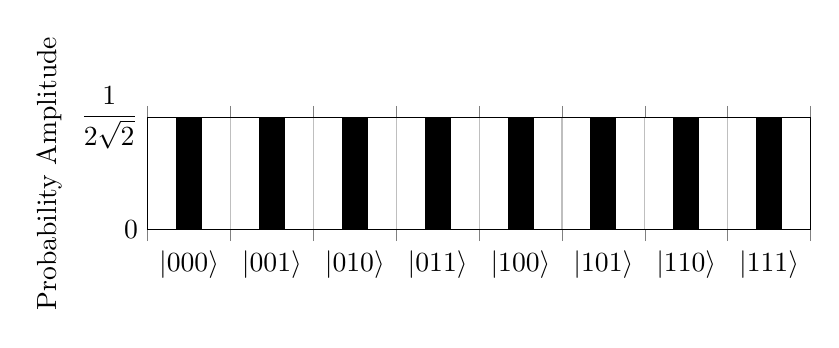
\begin{tikzpicture}
        \begin{axis}[
        width=10cm,height=3cm,
            x tick label style={/pgf/number format/1000 sep=},
            ymin=0,
            ymax=4,
            xmin=$\ket{000}$,
            xmax=6,
            ytick={0,4},
yticklabels={0,$\dfrac{1}{2\sqrt{2}}$},
            ylabel=Probability Amplitude,
            legend style={at={(0.5,-0.1)},anchor=north,legend columns=-1},
            ybar interval=0.3,
            symbolic x coords = {$\ket{000}$, $\ket{001}$, $\ket{010}$, $\ket{011}$, $\ket{100}$, $\ket{101}$, $\ket{110}$,$\ket{111}$,6,0}            
        ]
        \addplot [color=black,fill=black] coordinates {($\ket{000}$,4) ($\ket{001}$,4) ($\ket{010}$,4) ($\ket{011}$,4) ($\ket{100}$,4) ($\ket{101}$,4) ($\ket{110}$,4)($\ket{111}$,4) (6,0)};        
        \draw ({rel axis cs:0,0}|-{axis cs:0,0}) -- ({rel axis cs:1,0}|-{axis cs:0,0});
\draw ({rel axis cs:0,0}-|{axis cs:0,0}) -- ({rel axis cs:0,1}-|{axis cs:0,0});
        \end{axis}
\end{tikzpicture}
\end{center}
\centering 
\caption{Visualisation of the state at the start of Grover's Algorithm}
\end{figure}

A function called the quantum oracle then looks at the state and turns the probability amplitude of the desired section negative. It does this through the process $\ket{x}\rightarrow(-1)^{f(x)}\ket{x}$ where f(x)=1 on the part of the superposition related to the desired element and f(x)=0 otherwise. More precisely, this creates the superposition 
$\dfrac{1}{\sqrt{2}}(\ket{x}\ket{f(x)}-\ket{x}\ket{1 \oplus f(x)})$ The consequence of this is that a negative value will be returned when f(x)=1 and a positive value will be returned when f(x)=0.



 This process will inverse the probability amplitude of the desired element, resulting in the state below attempting to search for $\ket{101}$.
  \begin{figure}[H]
\begin{center}
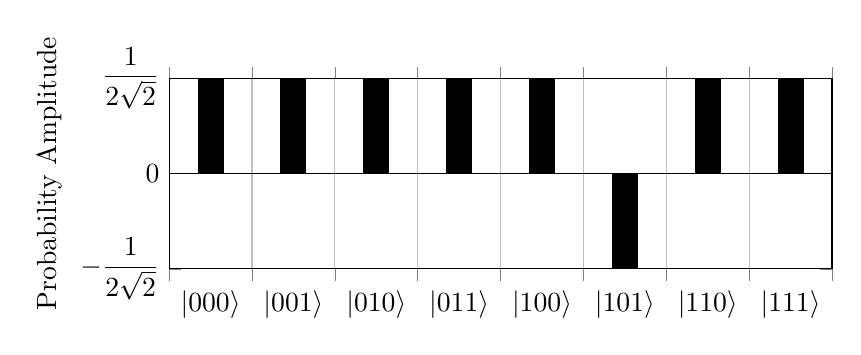
\begin{tikzpicture}
        \begin{axis}[
        width=10cm,height=4cm,
        ymin=-4,
        ymax=4,
        xmin=$\ket{000}$,
        xmax=6,
        x tick label style={/pgf/number format/1000 sep=},
        ytick={-4,0,4},
		yticklabels={$-\dfrac{1}{2\sqrt{2}}$,0,$\dfrac{1}{2\sqrt{2}}$},
        ylabel=Probability Amplitude,
        legend style={at={(0.5,-0.1)},anchor=north,legend columns=-1},
        ybar interval=0.3,
        symbolic x coords = {$\ket{000}$, $\ket{001}$, $\ket{010}$, $\ket{011}$, $\ket{100}$, $\ket{101}$, $\ket{110}$,$\ket{111}$,6,0}            
        ]
        \addplot [color=black,fill=black] coordinates {($\ket{000}$,4) ($\ket{001}$,4) ($\ket{010}$,4) ($\ket{011}$,4) ($\ket{100}$,4) ($\ket{101}$,-4) ($\ket{110}$,4)($\ket{111}$,4) (6,0)};        
        \draw ({rel axis cs:0,0}|-{axis cs:0,0}) -- ({rel axis cs:1,0}|-{axis cs:0,0});
\draw ({rel axis cs:0,0}-|{axis cs:0,0}) -- ({rel axis cs:0,1}-|{axis cs:0,0});
        \end{axis}
\end{tikzpicture}
\end{center}
\centering 
\caption{Visualisation after the oracle}
\end{figure}


After this, the states are then increased based on their difference from the mean and decreasing the amplitude if the difference is negative, resulting in a higher probability for the desired element.
  \begin{figure}[H]
\begin{center}
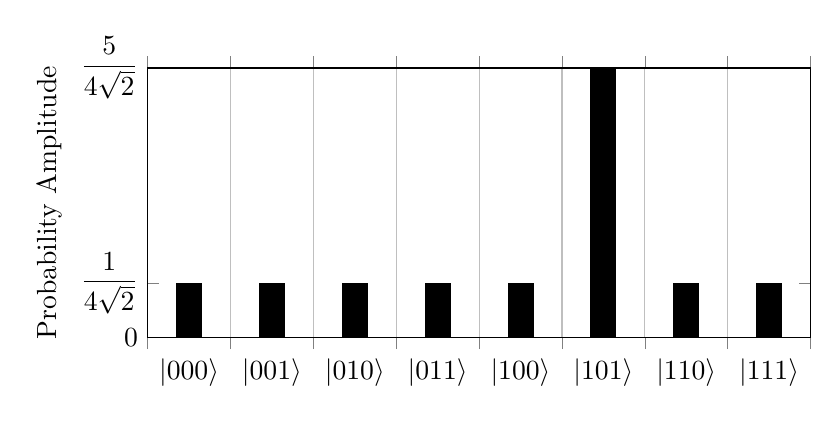
\begin{tikzpicture}
        \begin{axis}[
        width=10cm,height=5cm,
        ymax=5,
        ymin=0,
        xmin=$\ket{000}$,
        xmax=6,
            x tick label style={/pgf/number format/1000 sep=},
            ytick={0,1,5},
yticklabels={0,$\dfrac{1}{4\sqrt{2}}$,$\dfrac{5}{4\sqrt{2}}$},
            ylabel=Probability Amplitude,
            legend style={at={(0.5,-0.1)},anchor=north,legend columns=-1},
            ybar interval=0.3,
            symbolic x coords = {$\ket{000}$, $\ket{001}$, $\ket{010}$, $\ket{011}$, $\ket{100}$, $\ket{101}$, $\ket{110}$,$\ket{111}$,6,0}            
        ]
        \addplot [color=black,fill=black] coordinates {($\ket{000}$,1) ($\ket{001}$,1) ($\ket{010}$,1) ($\ket{011}$,1) ($\ket{100}$,1) ($\ket{101}$,5) ($\ket{110}$,1)($\ket{111}$,1) (6,0)};        
        \draw ({rel axis cs:0,0}|-{axis cs:0,0}) -- ({rel axis cs:1,0}|-{axis cs:0,0});
\draw ({rel axis cs:0,0}-|{axis cs:0,0}) -- ({rel axis cs:0,1}-|{axis cs:0,0});
        \end{axis}
\end{tikzpicture}
\end{center}
\centering 
\caption{Visualisation after transformation around the mean}
\end{figure}

After one run this has a probability of the desired element being measured of $\bigg(\dfrac{5}{4\sqrt{2}}\bigg)^2=\dfrac{25}{32}$, this puts the answer at a 78$\%$ probability of being correct when measured. In order to increase accuracy, this process is run $\dfrac{\pi}{4}\sqrt{2^N}$ times where N is the string length. For this example it would be $\dfrac{\pi}{4}\sqrt{2^3} = 2$ times. This would mean that another loop of the inversion around zero, followed by the transformation around the mean, would be required to improve it to a suitable level of accuracy. This would then result in a probability amplitude of $\dfrac{11}{8\sqrt{2}}$ for the correct element, giving a probability of 95$\%$, a much better success rate making the algorithm more reliable.

%\paragraph{Re-Do of Grovers}
%Grover's algorithm is a search algorithm for unordered lists, it does this by making the probability amplitude of the element to be searched for larger than the probability amplitude of all the other elements, making it a more likely result to come up.
%
%To perform this algorithm, initialise two qubits, Qubit 1 and Qubit 2. Apply the Hadamard transform to qubit 1 and apply the pauli X operator followed by the Hadamard transform to Qubit 2. Input this into the Quantum oracle in the function $\mathcal{O}(\ket{x}\otimes\ket{-})$, which can be expanded to $\dfrac{1}{\sqrt{2}}(\mathcal{O}\ket{x}\ket{0}-\mathcal{O}\ket{x}\ket{1}$. This can the quantum oracle sets $f(x)=1$ when $x$ is the desired element and $f(x)=0$ for all other elements. This means the function can be simplified to $\dfrac{1}{\sqrt{2}}(\ket{x}\ket{f(x)}-\ket{x}\ket{1\oplus f(x)})$. If f(x)=1 this can be simplified to $\dfrac{1}{\sqrt{2}}(\ket{x}\ket{1}-\ket{x}\ket{0})$ which is equal to $-\ket{x}\ket{-}$ which means that the probability amplitude of Qubit 1 has been inverted. If f(x)=0 it gives a result of $\ket{x}\ket{-}$, meaning that the state has not been changed.

\subsection{Grover's Algorithm compared to binary search}
 
The main advantage of Grover's Algorithm is that it can work on unordered lists, meaning that unlike binary search the list does not need sorting before an element can be found. The major advantage of this is that it does not also require a sorting algorithm and so is a much quicker option, meaning for larger databases it could be far superior. For large databases the extra storage required to hold the sorted data could mean that in binary search there would be a significant increase in storage costs as their requirements would in effect double if the data was not wanted to be stored in a sorted form. Another advantage of this is that the order of the data is often very important, and so by sorting it, the importance of the data is then lost. 
\\
\\
 The advantages of binary search are that it is a much quicker system to implement and is currently used in many facilities. This is because binary search can run on a classical computer, which is much cheaper both to buy and run than the quantum computer needed for Grover's algorithm.
\\
\\
Another advantage of binary search is that it can be used on explicit databases (databases spread over multiple storage areas) \autocite{practicalgrover} whereas Grover's algorithm cannot. This means that it is limited to a file stored in one place, vastly limiting its capability, as most large databases (an area where Grover's algorithm would be useful) are spread over multiple servers.For example, the millions of servers used by Google because it is impractical to store all the information in one place due to its size. Storing all the data in one place also reduces security and increases the impact of outages.
\\
\\
Binary search will also always give a correct answer, as opposed to the 90$\%$-100$\%$ accuracy of Grover's algorithm. This could be a large problem for large firms as a 10$\%$ failure rate over millions of searches would be unacceptable and so would mean that a classical algorithm would be the only option. 

 \section{Factoring Algorithms}
 \subsection{RSA Encryption}
 The main use of factoring numbers is in encryption, this is because many encryption systems work on the factors of large numbers, I will explore this with the example of RSA.
 RSA encryption works by multiplying two large prime numbers together, this creates the number, n.
 This n is then used to encrypt a message using the form $E=m^emod(n)$ where e is an encrypting value. This is then decrypted using $m=E^dmod(n)$. A value denoted as $\phi(n)$ is a value based on the factors of n found by $(p-1)\times(q-1)$ where p and q are the factors. This value of $\phi(n)$ is then used to find e as it is any number less than n that is not a factor. The value of d is then found using $\dfrac{k\times\phi(n)+1}{e}$ where k is the first integer that makes d an integer value. 
\\
RSA can be broken by finding the prime factors of n. This then allows for $\phi(n)$ to be found, allowing for d to be found, as shown above. Then with the message,E,the decrypting value, d, and n the message can be decrypted.
 
\subsection{Quadratic Sieve}
The quadratic sieve \autocite{sieve} is a classical algorithm used to factor numbers, it is performed by expressing the number to be factorised as the difference of two squares.
Starting at $\sqrt{N}$ and increasing the value of x until $x^2-N=y^2$ as below in factorisation of 989
  \begin{figure}[H]
\begin{center}
\begin{tabular}{ c|c|c}
x&$y^2$&y\\
\hline
32&35&5.916\\
33&100&10

\end{tabular}
\end{center}
\centering 
\caption{Quadratic Sieve}
\end{figure}
Obviously, not all iterations of this will be as quick but this shows that $33^2-10^2$ is equal to 989, the factors can then be found from 33+10=43 and 33-10=23. However, this will not work for all numbers. Factors can also be computed from values $(y_1)^2$ and $(y_2)^2$  that are not square numbers but multiply together to give a square number and the corresponding $x_1$ and $x_2$. With A being $x_1 \times x_2$ and B being $\sqrt{y_1^2 \times y_2^2}$ The GCD of (A+B, N) and (A-B, N) are factors.

 \subsection{Shor's algorithm}
 Shor's algorithm \autocite{shor} is a quantum algorithm which also factorises numbers, however it performs it through a different method to the quadratic sieve. The first task is to find the period of $x^a mod n$ where x is any number, 2 in my example. A is then increased from 0. n is the number to be factored. This will then create a list of numbers when performed and the period is found where the pattern repeats itself. In my example I tried to factor 989, as also shown in the quadratic sieve section. This results in a period of 154. Another number is then calculated by dividing the period over 2, called z in the formula then doing $y=a^z mod n$, working to being $y=2^{77} mod989$ which results in y=300. From this number the GCD of (y+1,n) and (y-1,n) is calculated, these are easily calculated with Euclid's algorithm, a classical algorithm, demonstrated below, trying to calculate GCD(301,989) and GCD(299,989). For example for 301 and 989:
   \begin{figure}[H]
\begin{center}
989=301$\times$3+86\\
301=86$\times$3+43\\
86=43$\times$2+0
\end{center}
\centering 
\caption{Euclid's Algorithm}
\end{figure}
When the number is added, the greatest common divisor will be the number at the end above, in this example 43. Doing this again for the other two numbers gives 23, these two numbers are the prime factors of 989. This is how it is performed classically, however when trying to find the period of large numbers takes too much time. 
Shor's algorithm takes the number to be factored (N), and a random number (A) which is not a factor of N (GCD(N,A)=1). Another number, n, is chosen which dictates the size of the register, the larger this is the greater the time taken but the greater the accuracy. For this example N will be 39, A will be 7 and n will be 10. q is $2^n$ so in this case it is $2^{10}$.

The algorithm is started in the state $\ket{0}\ket{0}$, the QFT (Quantum Fourier Transform) is then applied to the first Qubit, changing it to the state:
   \begin{figure}[H]
\begin{center}
$\ket{\psi}=\dfrac{1}{\sqrt{q}}\sum\limits_{x=0}^{q-1}\ket{x}\ket{0}$
\end{center}
\centering 
\caption{Shor's Algorithm State 1}
\end{figure}
So with the numbers used in the example it is
   \begin{figure}[H]
\begin{center}
$\ket{\psi}=\dfrac{1}{2^5}\sum\limits_{x=0}^{{2^{10}}-1}\ket{x}\ket{0}$
\end{center}
\centering 
\caption{Shor's Algorithm State 2}
\end{figure}

Now $f(x)$ is calculated and put in the second register, in Shor's algorithm $f(x)$ is $a^x mod n$. This then creates the state
   \begin{figure}[H]
\begin{center}
$\ket{\psi}=\dfrac{1}{2^5}\sum\limits_{x=0}^{{2^{10}}-1}\ket{x}\ket{f(x)}$
\end{center}
\centering 
\caption{Shor's Algorithm State 3}
\end{figure}
The second qubit is then measured, this causes it to collapse to one state, meaning that the state will only include instances where f(x)=y, with y being the measured value. This now makes it easier to find the period, as the difference between values in the state is the period. The inverse QFT is then applied to this state.

This transformation then leads to a distribution of values with some having higher probability than others. The most likely values, divided by q, will approximately give a fraction, whose numerator is the period. For the numbers given above a likely value is 85. This is then divided by $2^{10}$ to give a fraction. This fraction is then converted, by continued fractions, into a number with a numerator of 1. This will give $\dfrac{1}{12}$, giving the period of 12. 

This period is then used in the formula $a^{r/2}modN$ which is $7^6mod39=25$ the GCD of (25-1,37) and (25+1,39) are then found which are 3 and 13, which are the prime factors of 39.

 \subsection{Shor's algorithm compared to Quadratic Sieve}
For the example of factoring a larger number, for example 792347. Shor's algorithm runs in \\
$(2logN)(loglogN)(logloglogN)$ time. This means that it will run in 68 time units. However, the quadratic sieve runs in $e^{\sqrt{\ln(n)\ln(n)\ln(n)}}$ time which would mean it would run in $5.4\times10^{21}$ time units. This difference is because quadratic sieve runs in exponential time, whereas Shor's algorithm runs in log time, meaning that as the number gets larger the difference in speed for Shor's will be less than the difference for the quadratic sieve. Factoring becomes interesting regarding cryptography, this is because one of the most popular encryption methods is RSA. The current largest RSA number is RSA-2048, this is 2048 bits, equal to 617 digits. Using general number field sieve, the fastest algorithm for strings over 100 digits long, the time taken would be $4.8\times10^{34}$ units. This is much longer than the run time for Shor's algorithm for that number, which would be 40884 time units. The potential of Shor's algorithm could mean that current cryptography systems will be obsolete as the security of RSA comes from the fact that the numbers can't be factored. Supposing that the time units were seconds, the classical algorithm would take longer than the life of the universe as it would take $1.5\times10^{27}$ years and the life of the universe is $1.1\times10^{17}$ years. Comparing this to the run time of Shor's algorithm which is 11 hours, it is easy to see the danger that Shor's algorithm poses to existing encryption.

\section{Conclusion}
In conclusion the physics of quantum computers allow for superior computation to classical computers, but they come with the trade-off of increased manufacturing costs, increased power consumption and increased space requirements compared to a classical computer
\\
\\
Due to the increased popularity and reduced complexity of classical computers compared to quantum computers, how they work is much more widely known. This allows for far more people to be able to work on them, making it a better choice for companies to use them. 
\\
\\
Quantum algorithms allow for data to be processed much faster than classical algorithms, however there is currently only a few available algorithms, meaning the utility of quantum computing is not yet fully realised. Quantum algorithms also are only superior to classical algorithms when processing large values, meaning that they wouldn't provide any noticeable benefit to domestic consumers and may even perform worse than classical computers, whose main use is lots of short processes.
\\
\\
Currently quantum computers are only experimental, but some large companies, such as NASA, have bought a quantum computer in order to see what practical uses they can offer. However, companies such as Google may soon be able to find a practical use for them, for example, improving the speed of their search results, meaning they would be able to reduce the number of traditional servers, saving both power and space. 
\\
Without any breakthrough development in cooling technology, or a way to operate a quantum computer at room temperature, it is unlikely that quantum computers will be used directly by consumers in the foreseeable future. Instead they will be used as a replacement for supercomputers due to their reduced space and power requirements for the same performance. Therefore the only interaction consumers will have with quantum computers will be over the internet. This is because they have the power to increase the speed and accuracy of image recognition, search speed and may also revolutionise the encryption industry. 
\\
\\
I believe I have achieved what I have set out to achieve as I explored the utility of quantum computers and their limitations. I think overall quantum computers could be better than supercomputers but it is unlikely they will be used, widely in the consumer market without further advances in technology.








\newpage

\printbibliography


 

\end{document}
